\begin{frame}{Fit invariant mass}
    \begin{columns}
        \begin{column}{.55\textwidth}
            \centering
            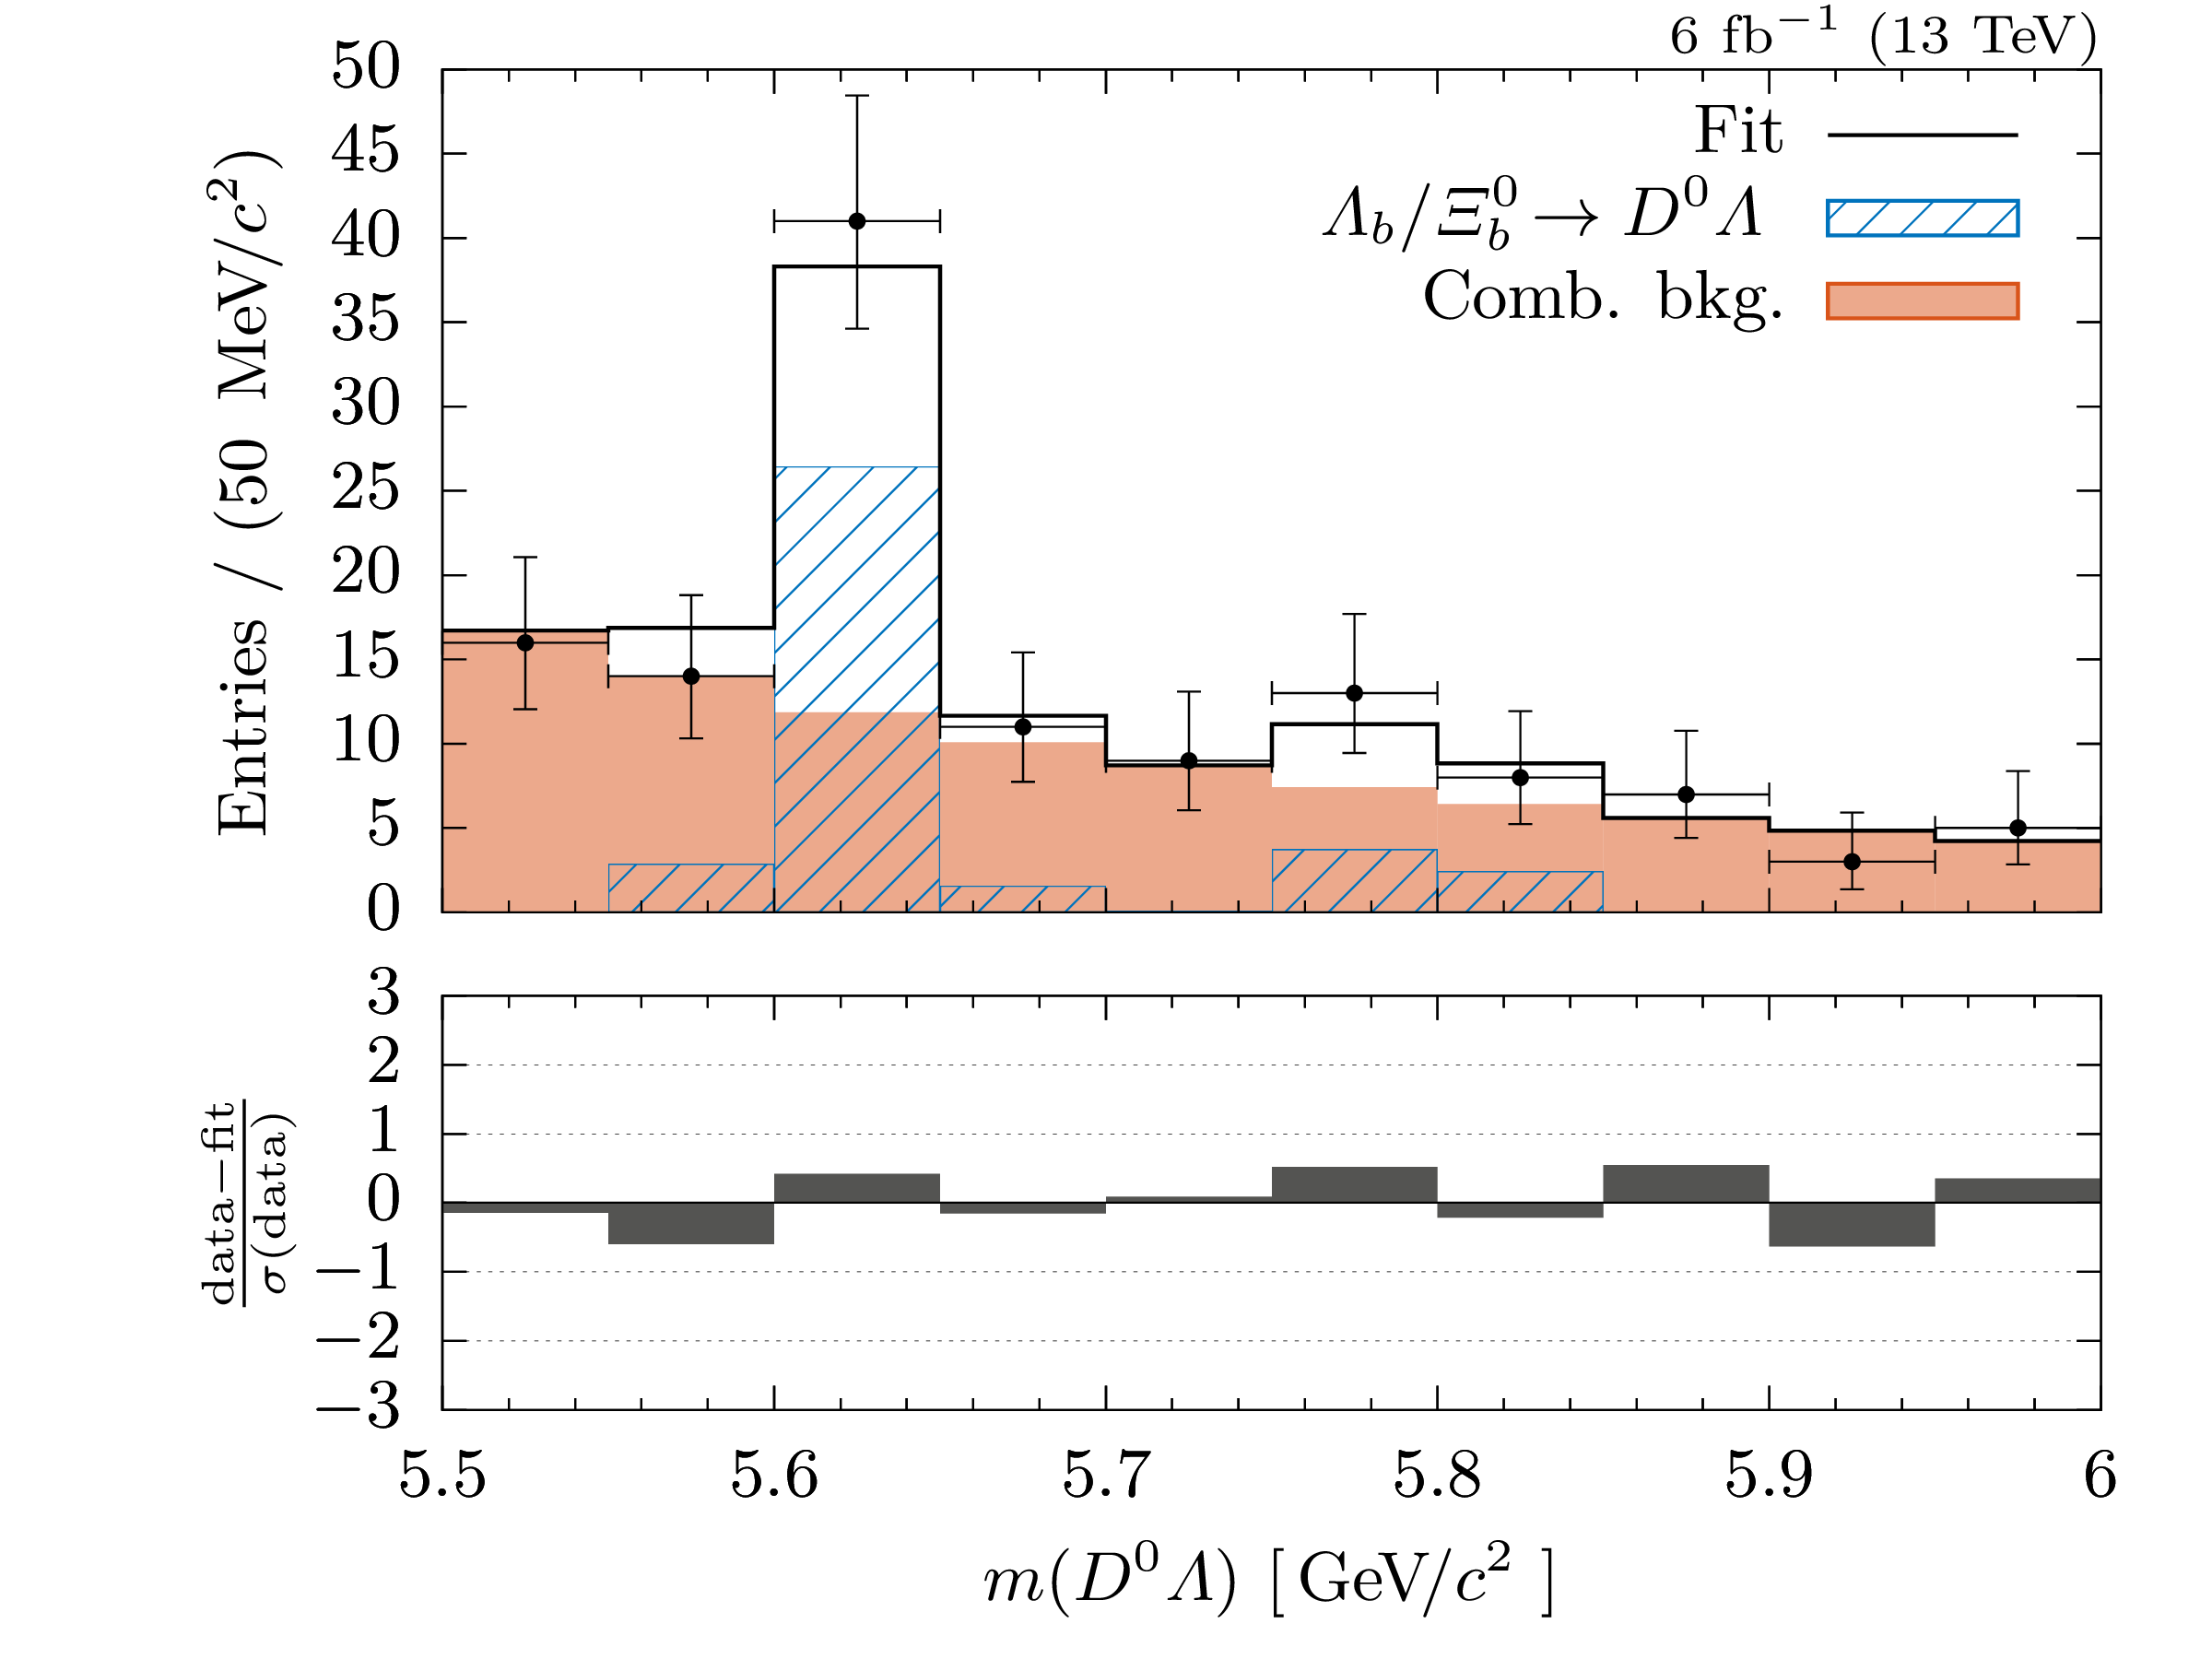
\includegraphics[width=\textwidth]{fit/hLbM_data_fit1.png}
            \textbf{Result:} $n(\Lb) = 31(7)$ and $n(\Xibz) = 6(4)$ \\ (\textcolor{vertexDarkRed}{only stat.\ uncertainty given})
        \end{column}
        \begin{column}{.45\textwidth}
            \begin{itemize}
                \item Fit remaining 260 signal candidates (rec.\ data)
                \item Simultaneously fit rec.\ and MC sim.\ data of both track types \\ (6 samples)
                \begin{itemize}
                    \item 23 parameters
                    \item most of them shared between at least two samples
                \end{itemize}
                \item Vary fit model to check for systematic error
                \begin{itemize}
                    \item change parametrization
                    \item change inv.\ mass range
                    \item \ldots{} (8 variations in total\ftntdagger)
                \end{itemize}
            \end{itemize}
        \end{column}
    \end{columns}
\end{frame}

\begin{frame}{Fit invariant mass}
    \begin{columns}
        \begin{column}{.55\textwidth}
            \centering
            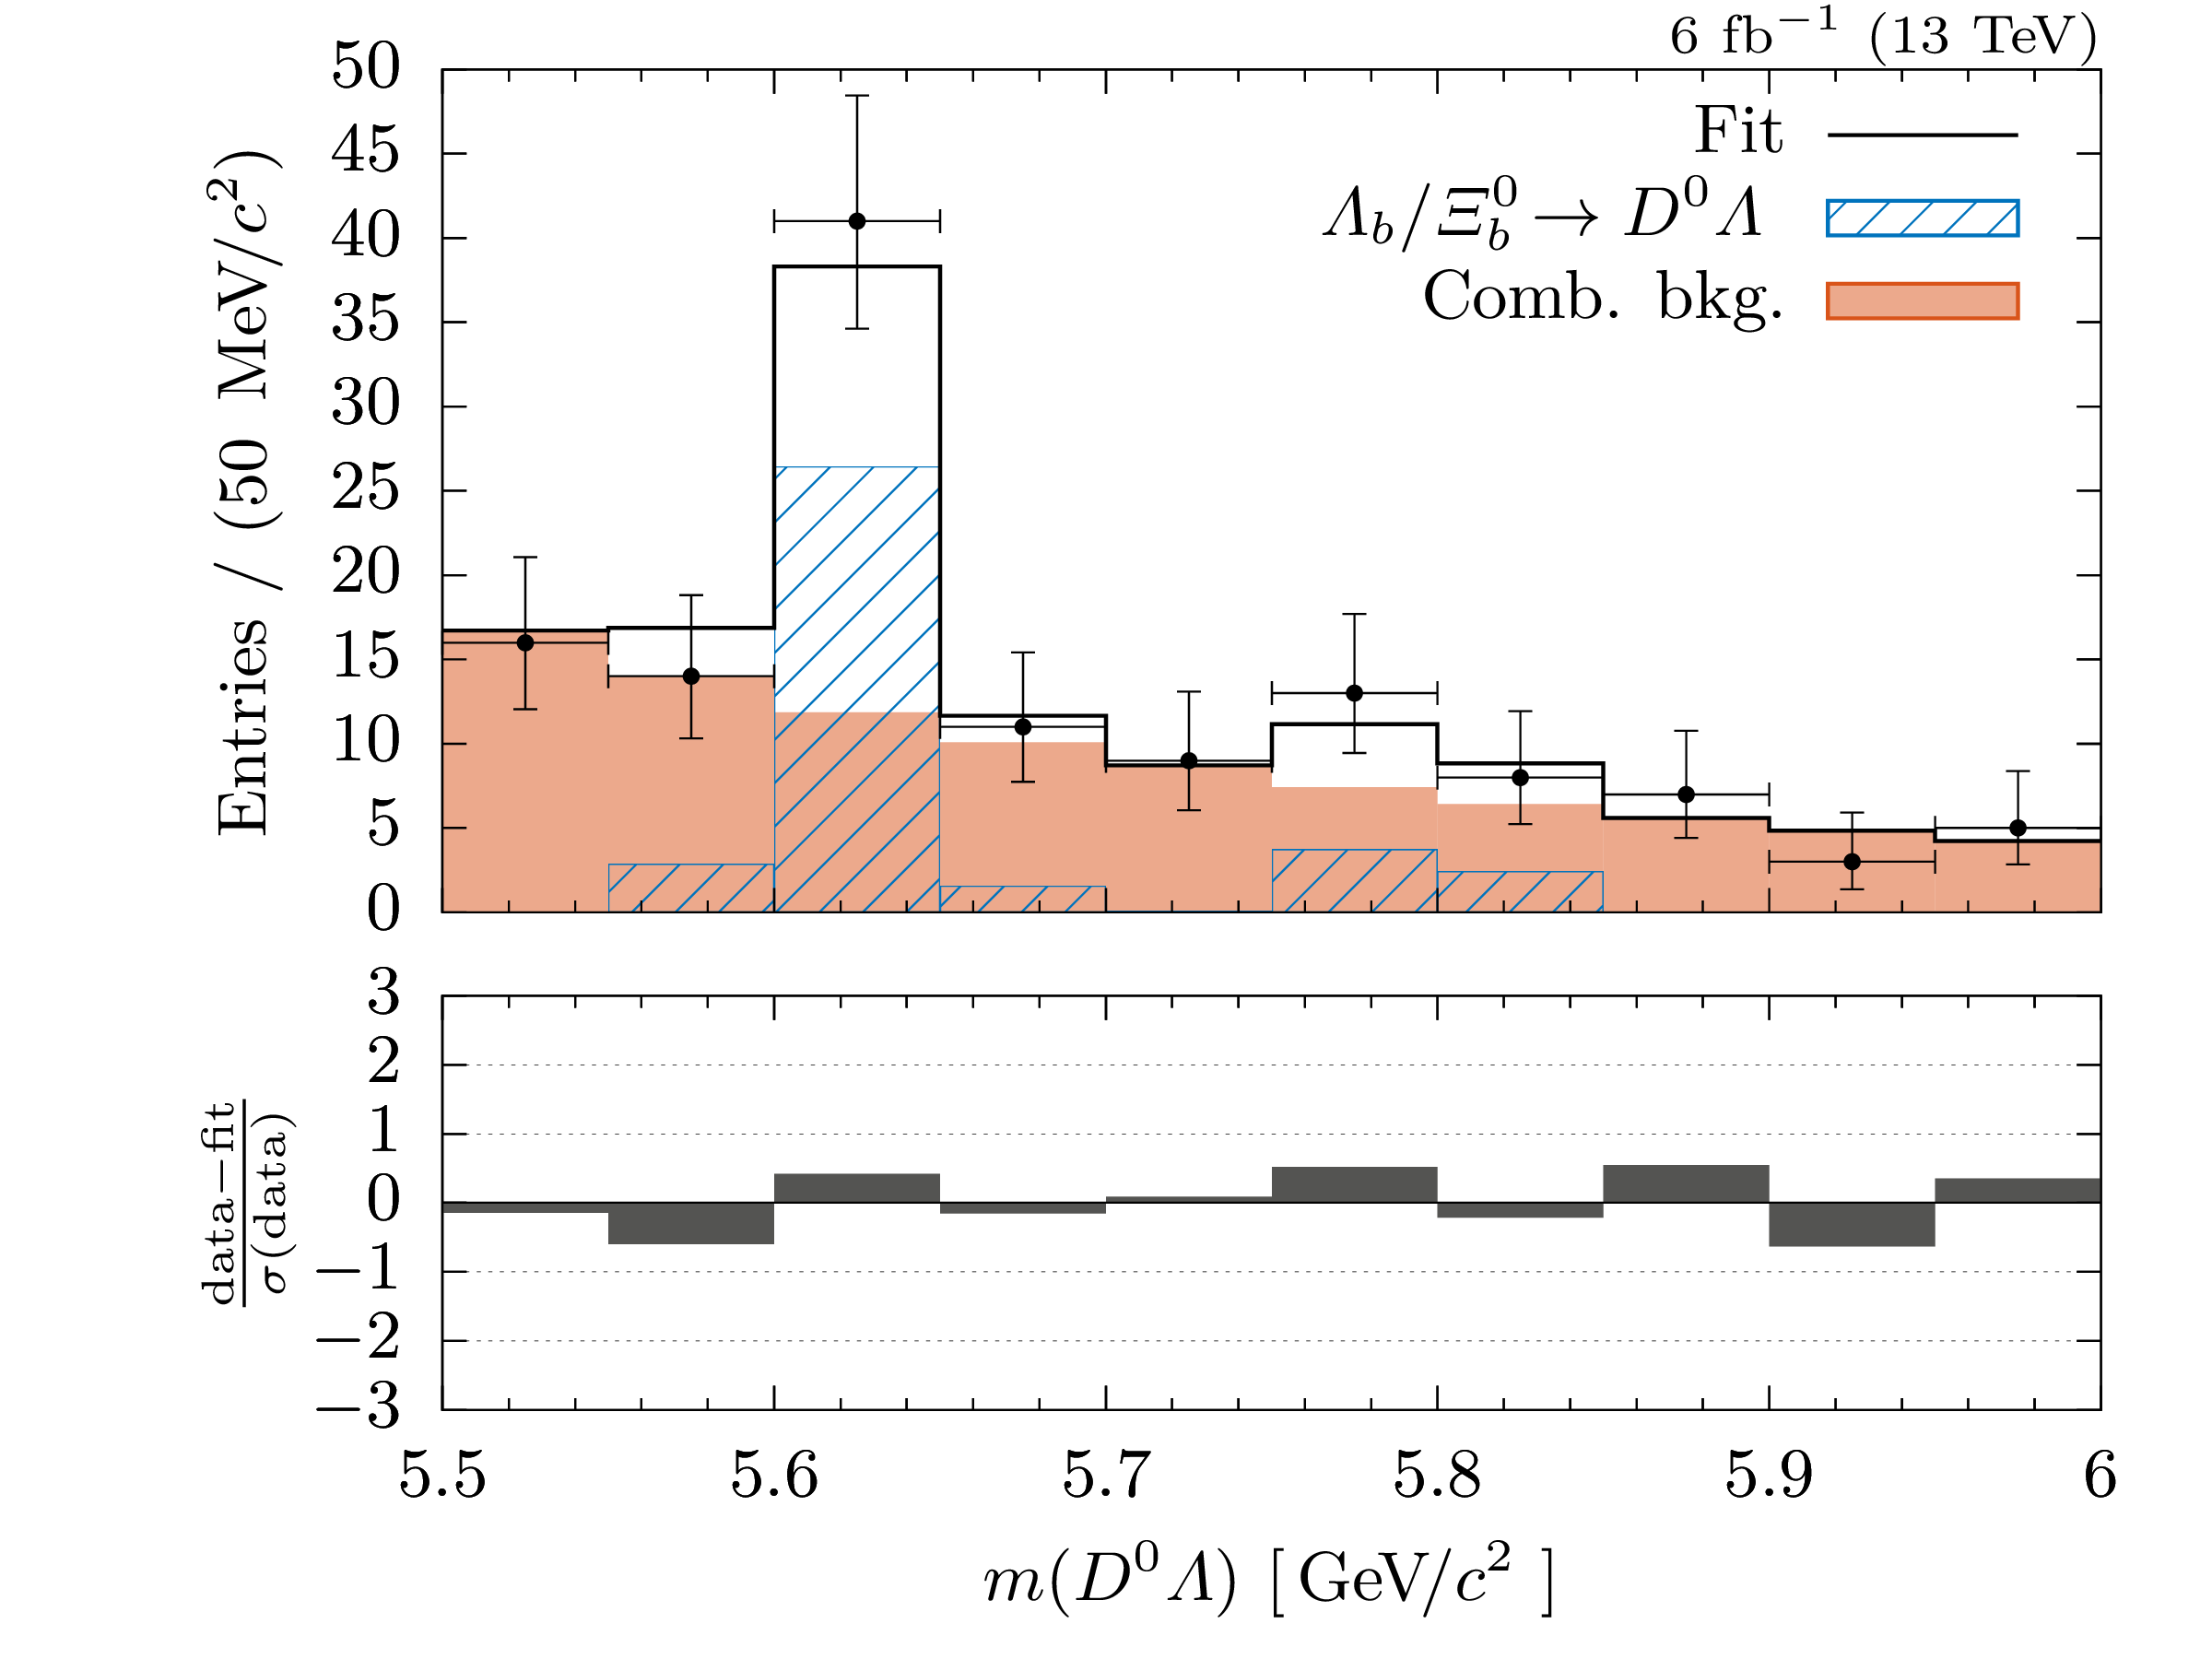
\includegraphics[width=\textwidth]{fit/hLbM_data_fit1.png}
            \textbf{Result:} $n(\Lb) = 31(7)$ and $n(\Xibz) = 6(4)$ \\ (\textcolor{vertexDarkRed}{only stat.\ uncertainty given})
        \end{column}
        \begin{column}{.45\textwidth}
            \only<1>{%
            \textbf{Sanity checks} 
            \begin{itemize}
                \item (Bias of estimated yields\ftntdagger)
                \item (Validity of (stat.) error estimates\ftntdagger)
            \end{itemize}}
            \only<2>{%
            \textbf{Stat.\ significance of yields} 
            \begin{itemize}
                \item Fix all parameters from MC sim.
                \item Run fit twice 
                \begin{itemize}
                    \item $\mathcal{L}$ for signal comp.\ \textbf{enabled}
                    \item $\mathcal{L}$ for signal comp.\ \textbf{disabled}
                \end{itemize}
                \item Stat.\ sign.\ given by $\sqrt{-2 \Delta \! \ln \mathcal{L}}$
            \end{itemize}}
        \end{column}
    \end{columns}
\end{frame}

\begin{frame}{Statistical significance of yields}
    \begin{columns}
        \begin{column}{.5\textwidth}
            \textbf{Wilks theorem}
            \begin{itemize}
                \item Here: \textcolor{vertexDarkRed}{if} sample size tends to infinity $2 \Delta\!\ln \mathcal{L}$ tends to a $\chi^2$-distribution with one DoF
                \item Hence: stat.\ significance of rej.\ null hypothesis \textit{no signal} is $\sqrt{-2 \Delta \! \ln \mathcal{L}}$
                \item Test assumption with pseudo experiment (\textit{Toy MC})
                \begin{itemize}
                    \item sample Toy MC from fitted PDF w/o signal component
                    \item run fit twice (w/ and w/o signal component)
                \end{itemize}
            \end{itemize}
        \end{column}
        \begin{column}{.5\textwidth}
            \centering
            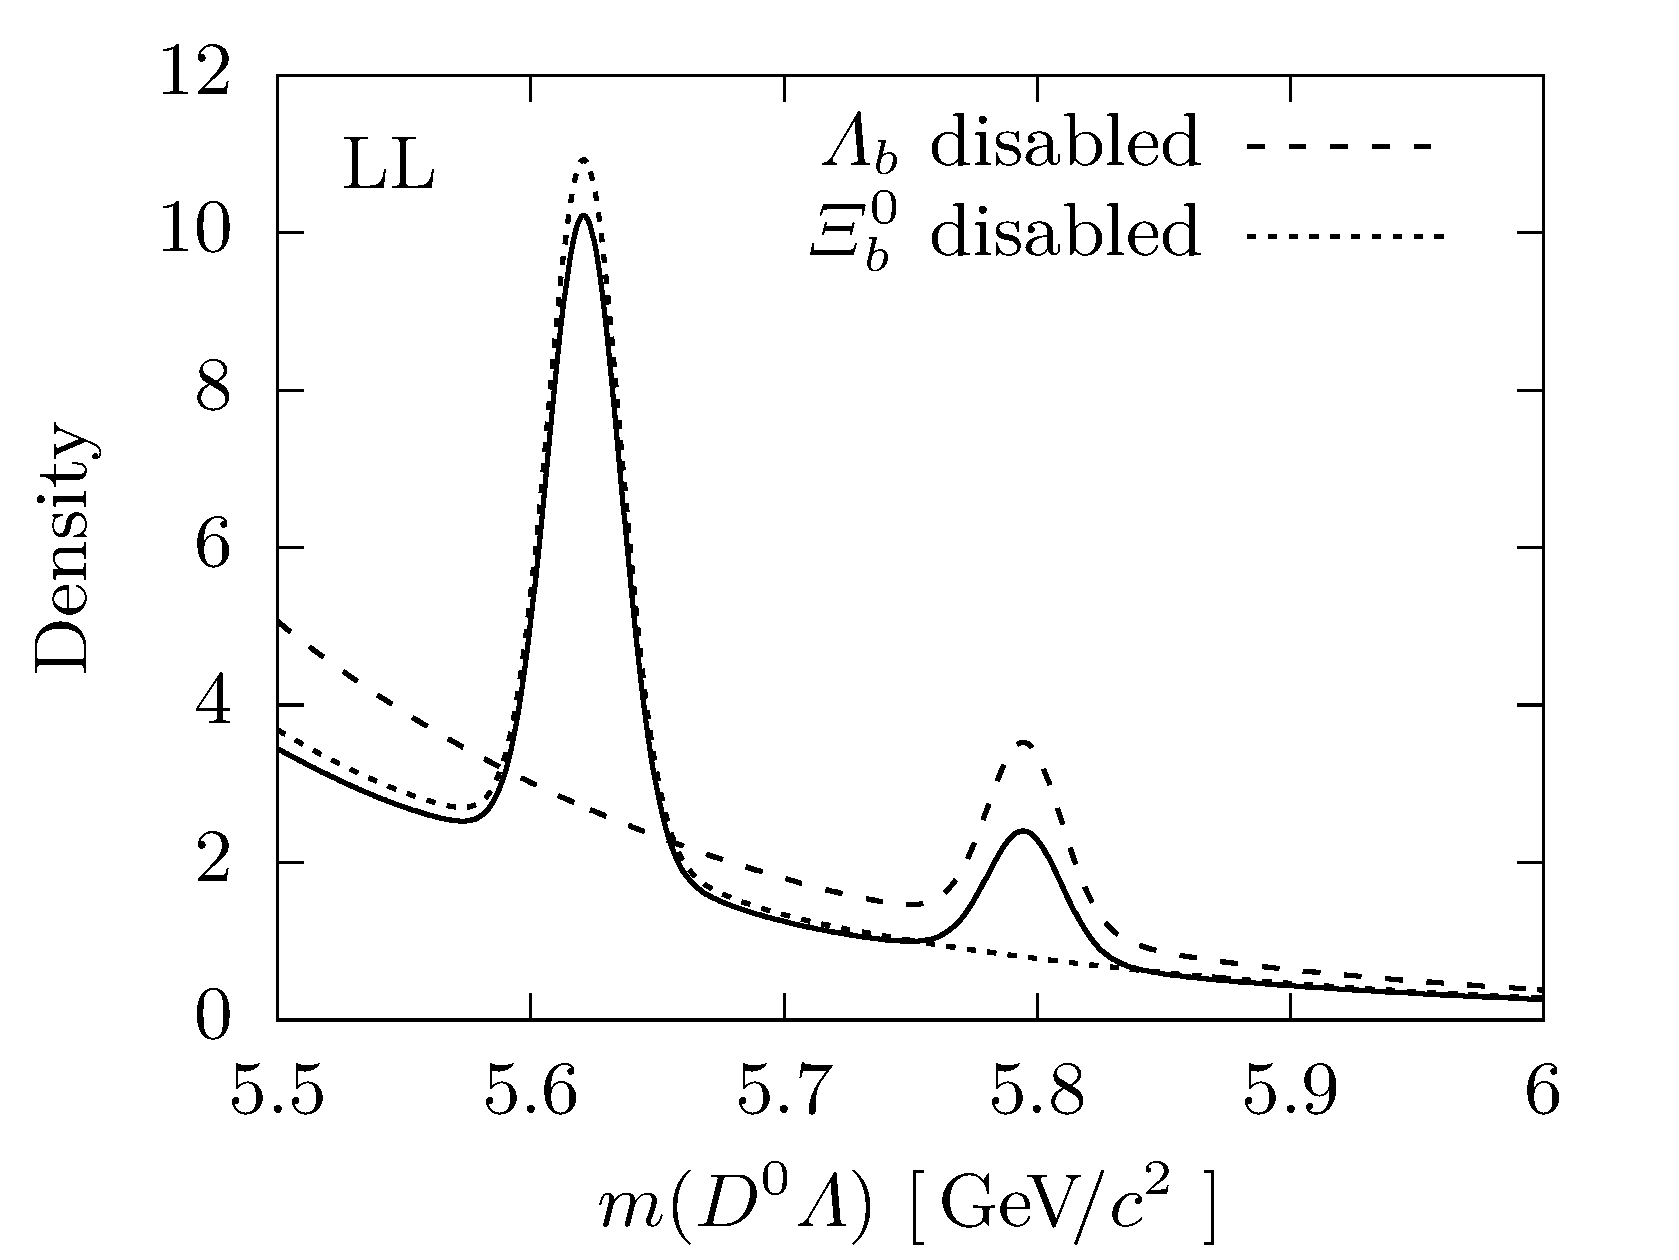
\includegraphics[width=\textwidth]{fit/pdf_LL.png}
        \end{column}
    \end{columns}
\end{frame}

\begin{frame}{Statistical significance of yields}
    \centering
    \only<1>{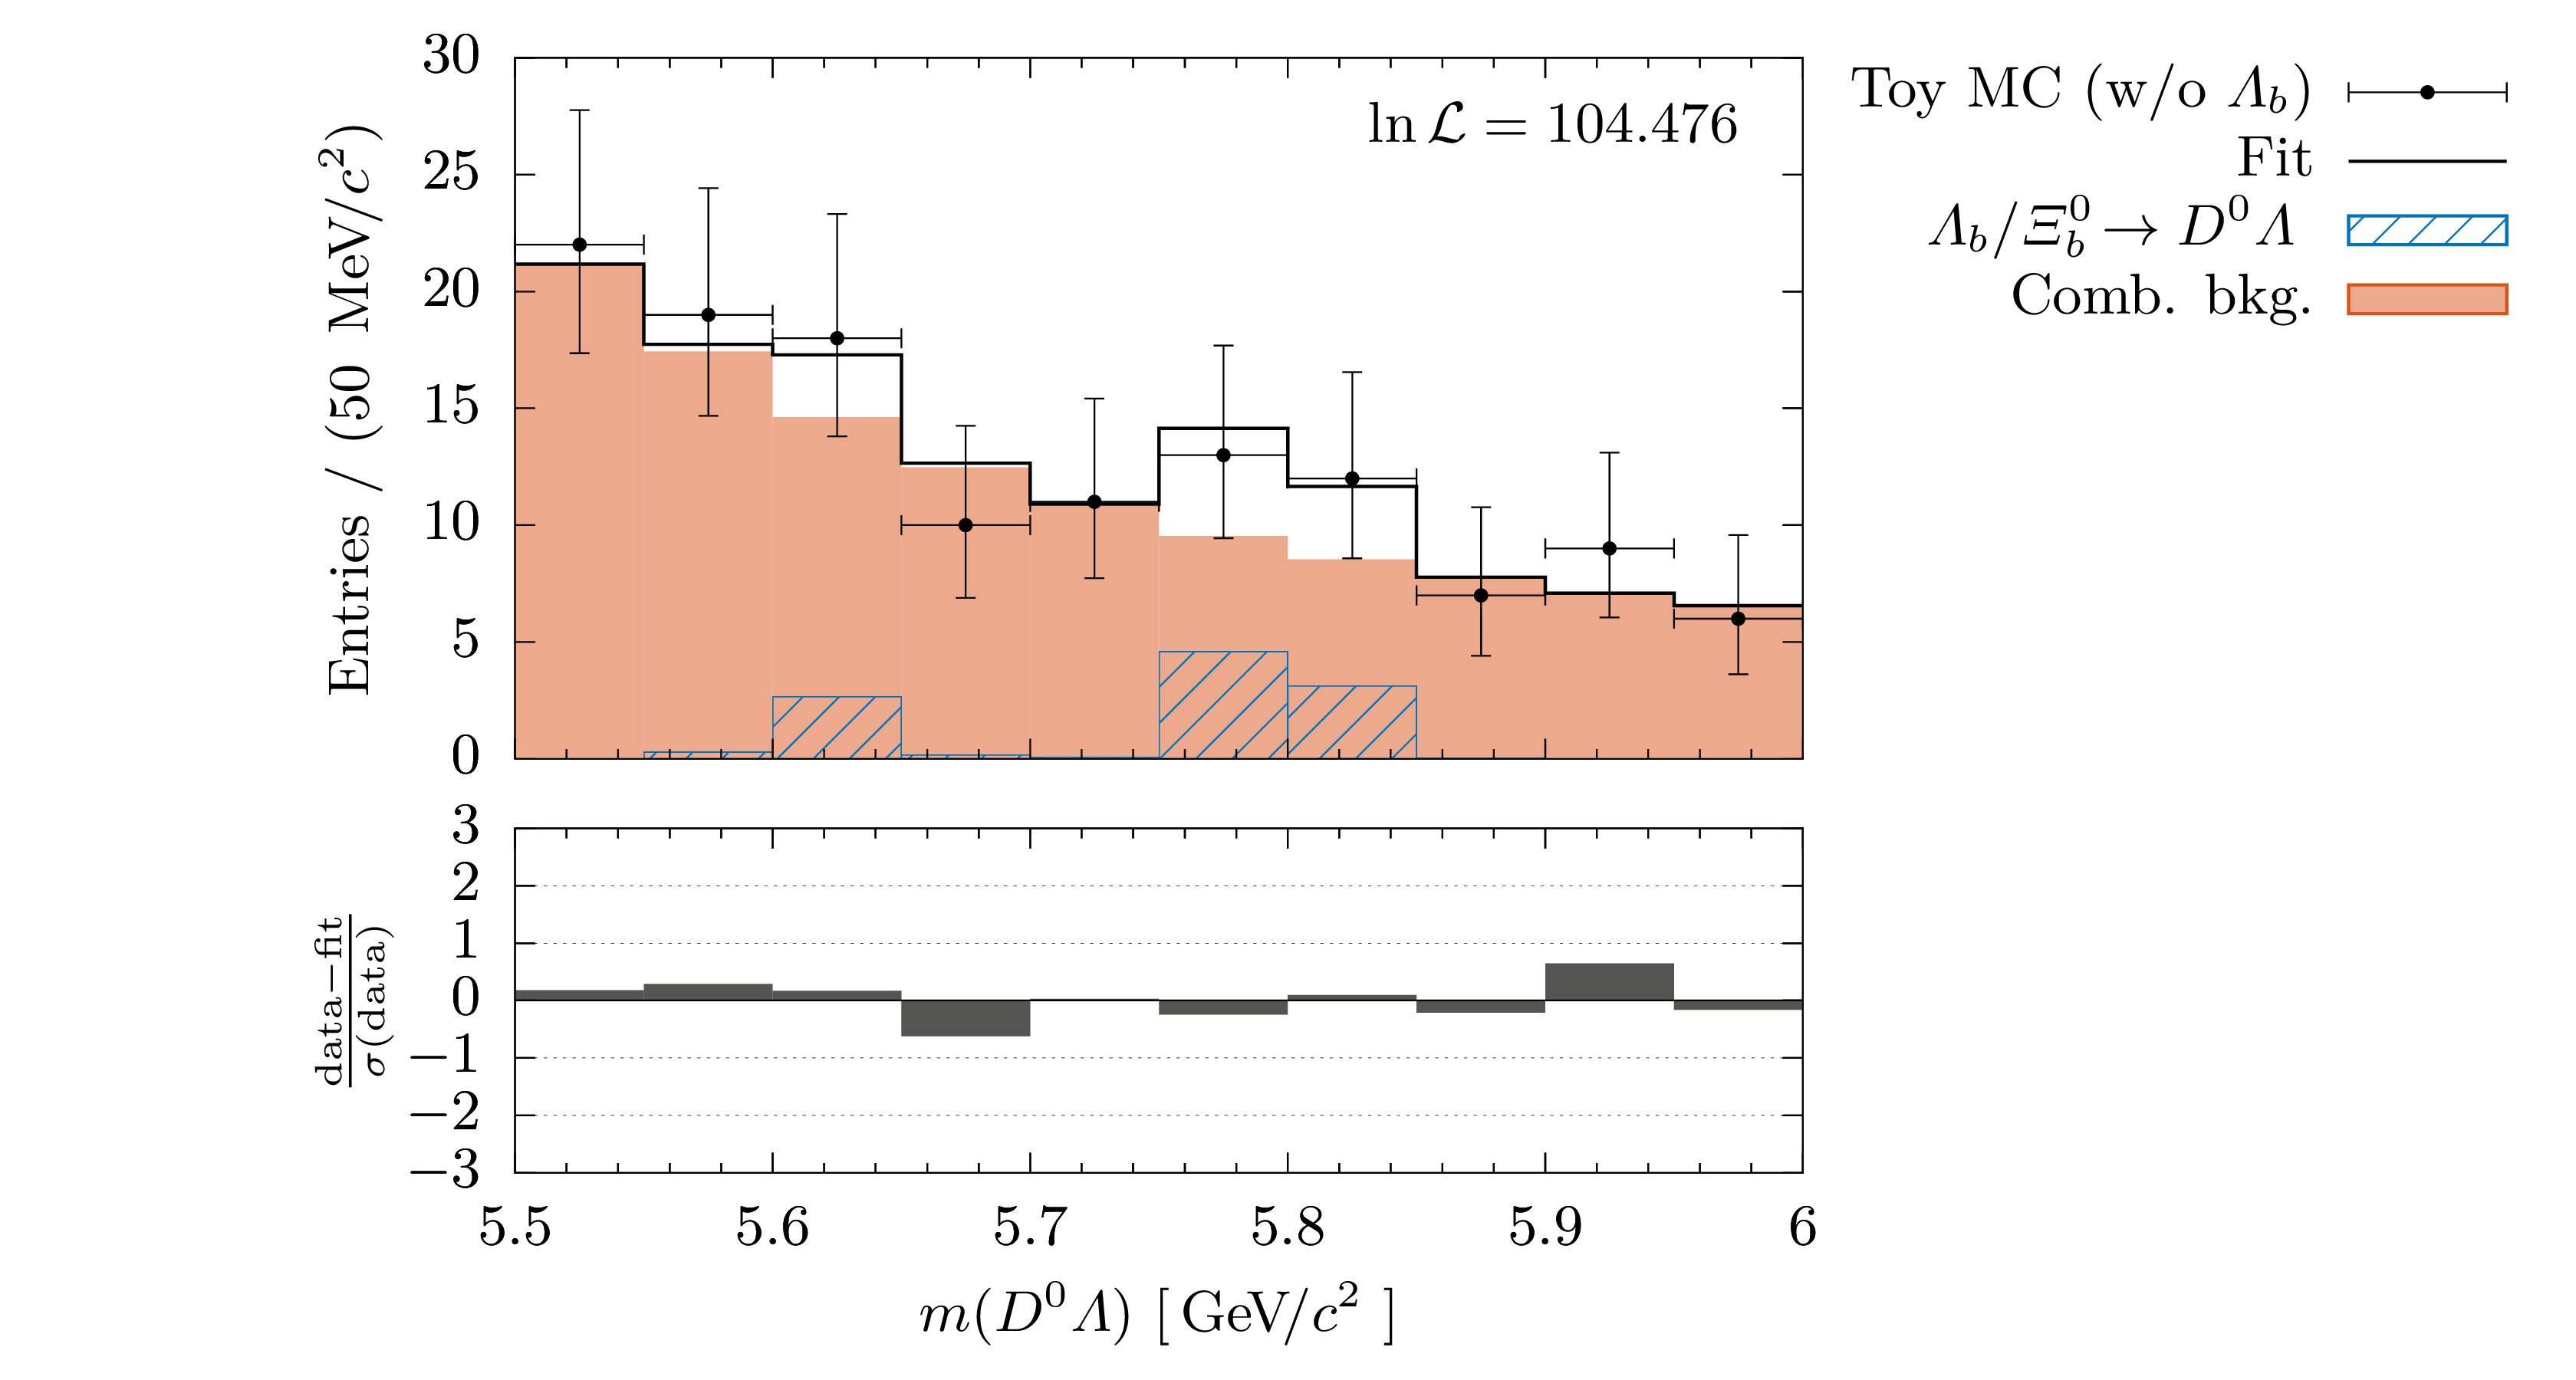
\includegraphics[scale=1.]{fit/hLbM_toy_noLb_fit1.png}}%
    \only<2>{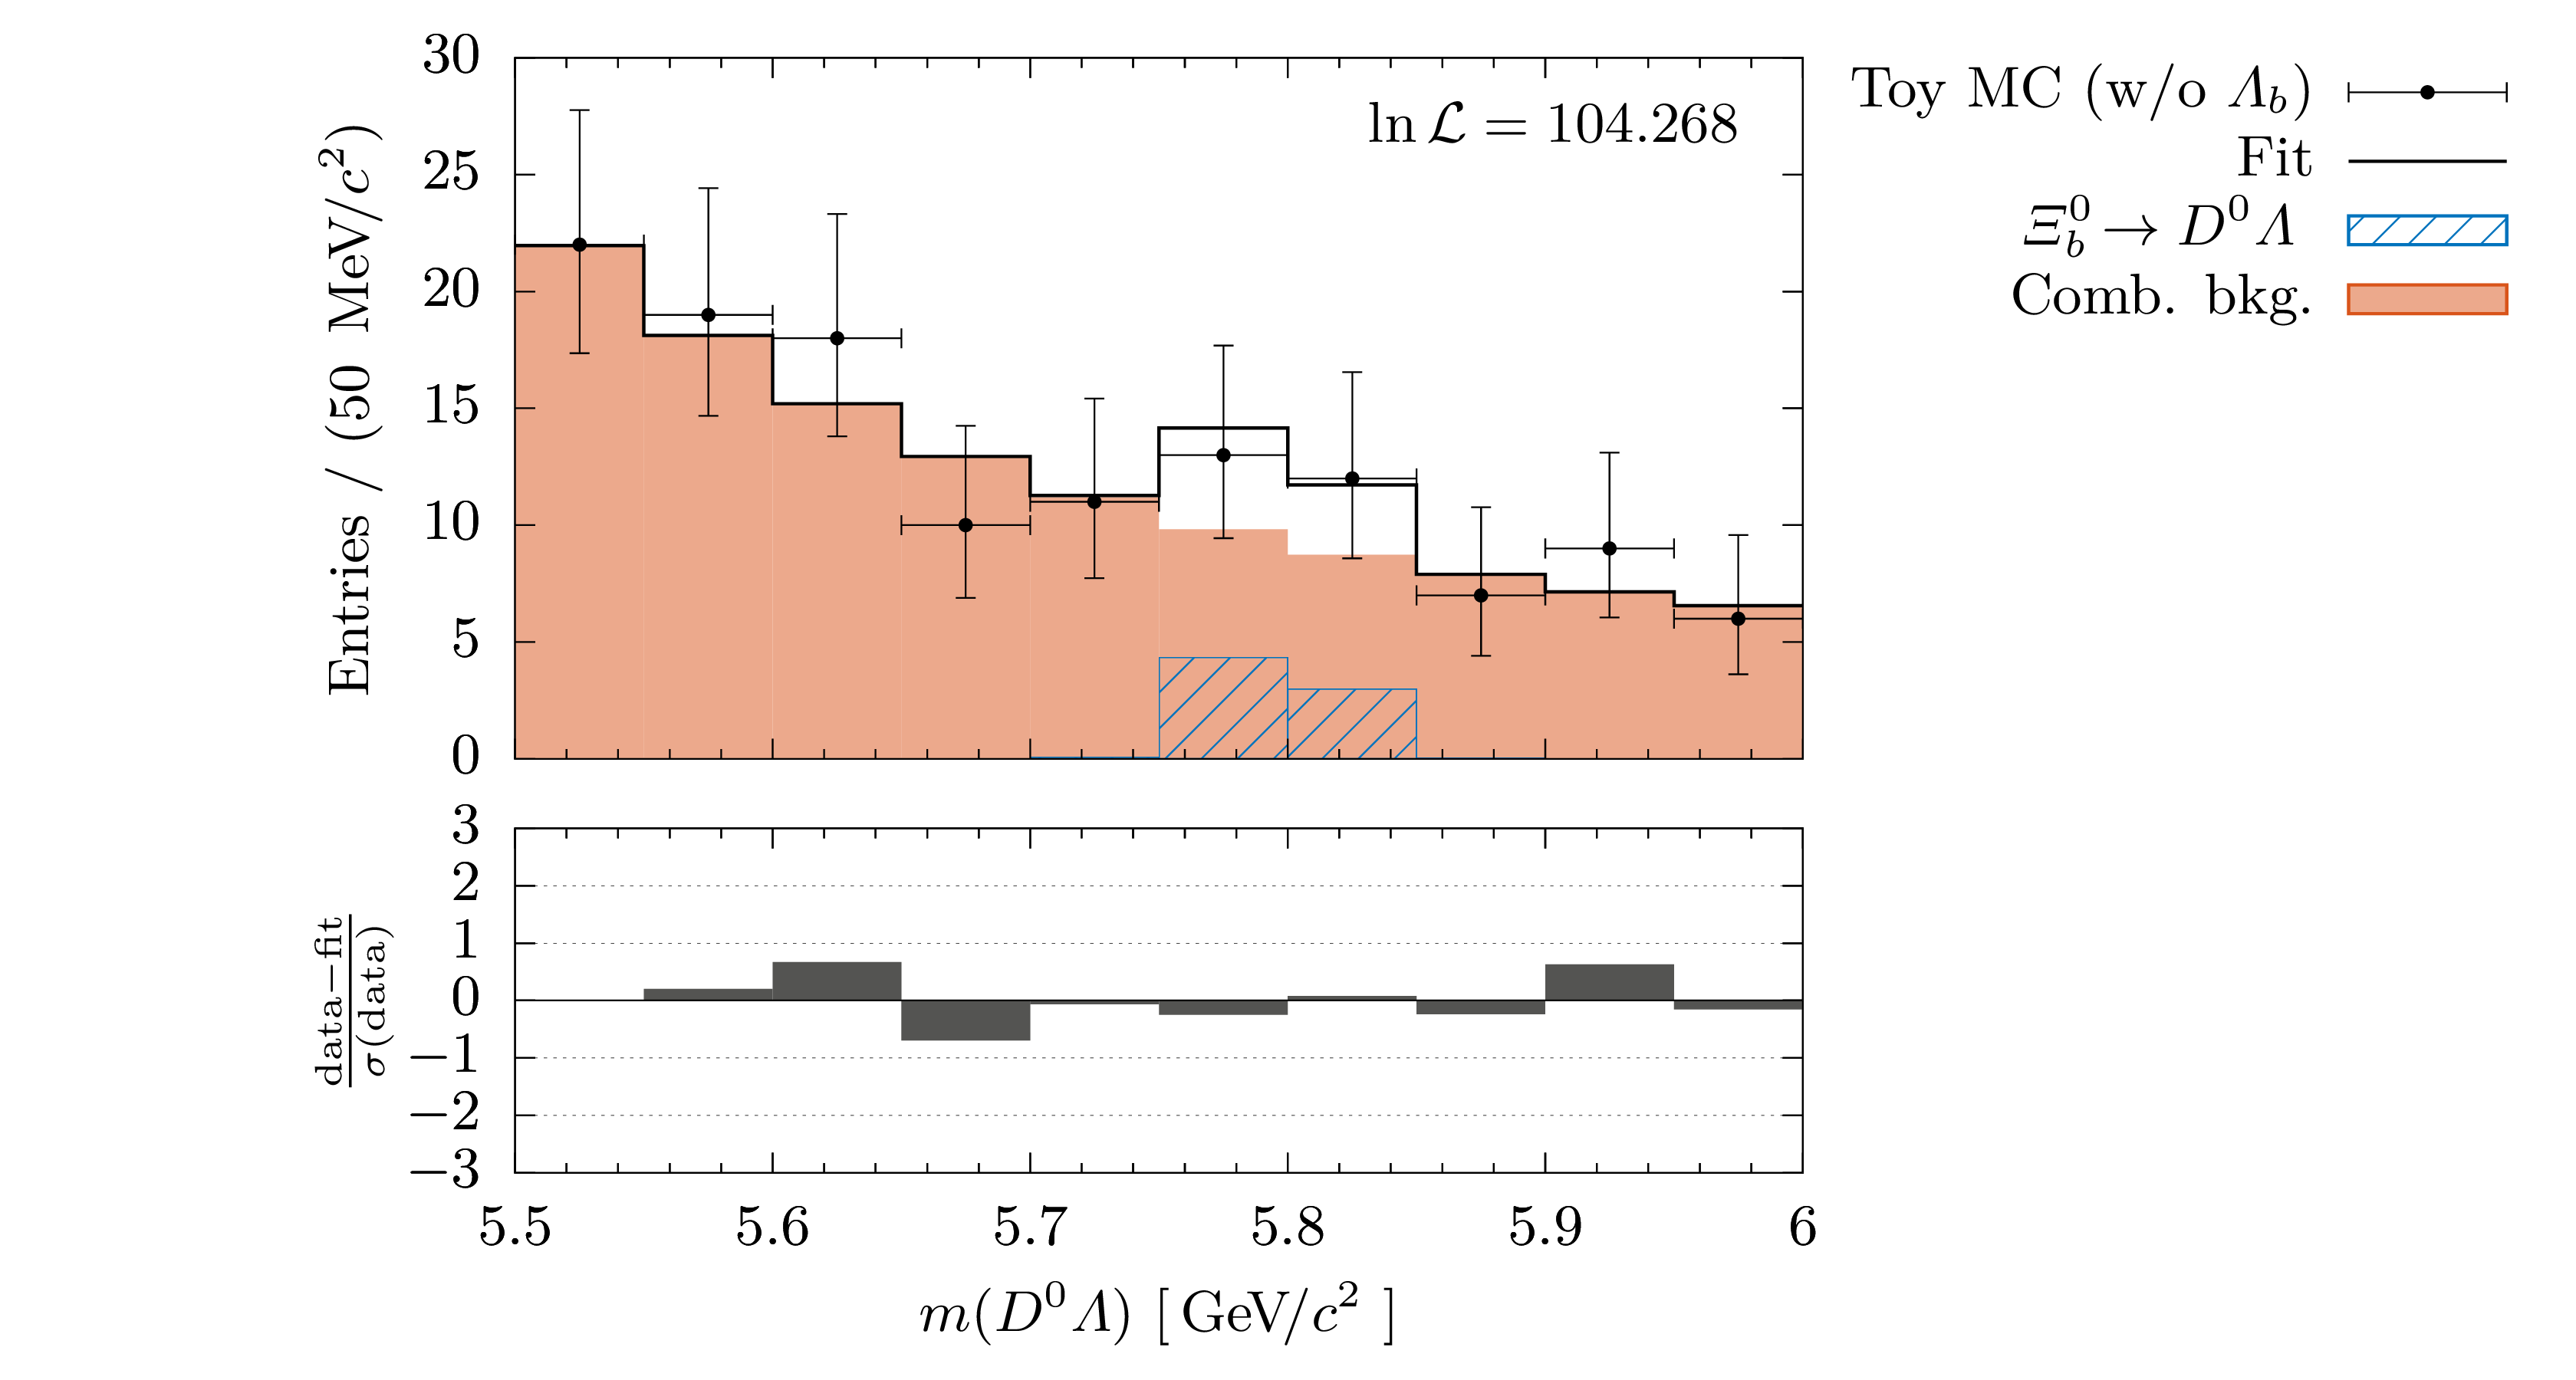
\includegraphics[scale=1.]{fit/hLbM_toy_noLb_fit2.png}}%
\end{frame}

\begin{frame}{Statistical significance of yields}
    \centering
    \only<1>{\begin{overpic}[scale=1.]{fit/hLbM_data_fit2_2.png}
        \put(70,52){\colorbox{white}{\phantom{xxxxxxxxxxxx}}}
        \put(68,52){$\ln \mathcal{L} = 106.569$}
    \end{overpic}}%
    \only<2>{\begin{overpic}[scale=1.]{fit/hLbM_data_fit1.png}
        \put(68,52){$\ln \mathcal{L} = 121.944$}
    \end{overpic}}%
\end{frame}

\begin{frame}{Statistical significance of yields}
    \begin{columns}
        \begin{column}{.5\textwidth}
            \centering
            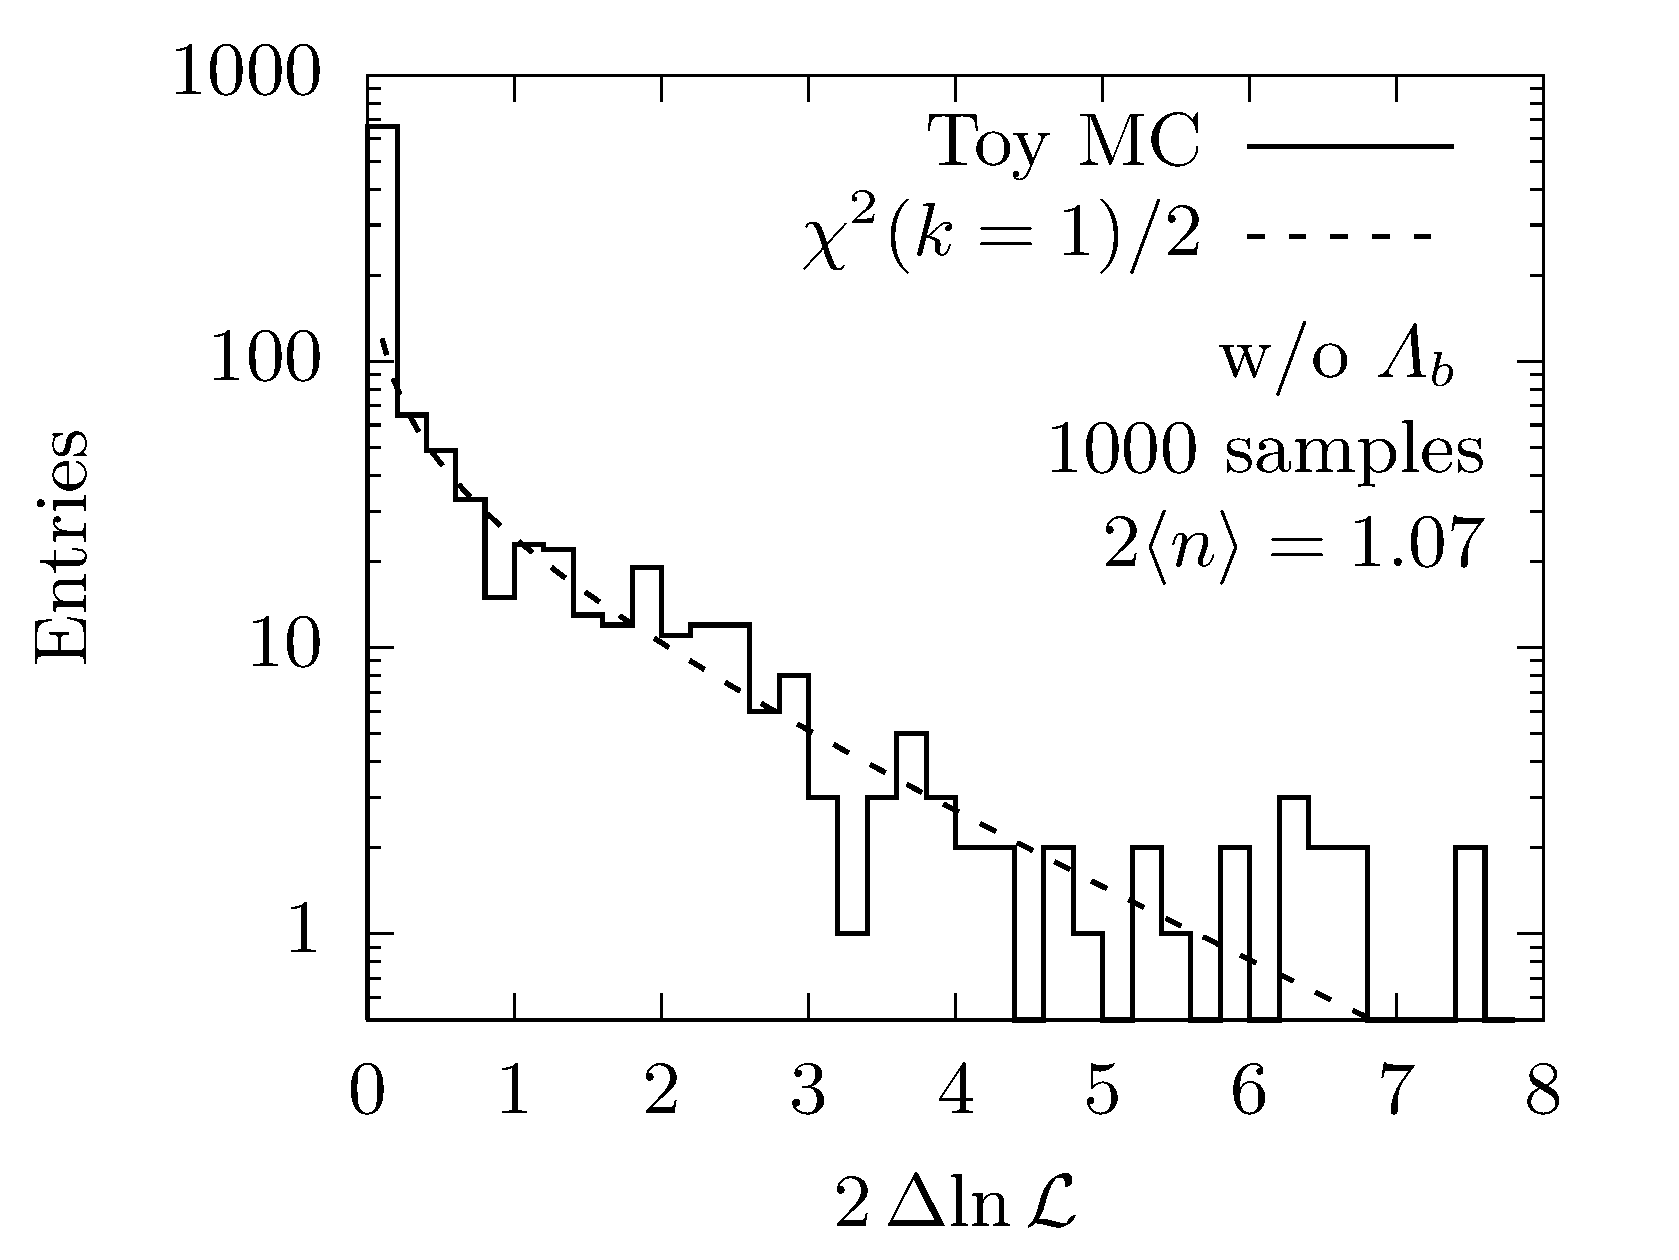
\includegraphics[width=\textwidth]{fit/deltaL_noLb.png}
        \end{column}
        \begin{column}{.5\textwidth}
            \textbf{Wilks theorem}
            \begin{itemize}
                \item Distribution of $\Delta \!\ln \mathcal{L}$ indeed follows a $\chi^2$-distribution with 1 DoF
                \item Wilks theorem is applicable!
            \end{itemize}
        \end{column}
    \end{columns}

    \vspace{5mm}
    
    \centering
    \scalebox{1.2}{Estimated \textbf{yield significances}: \textcolor{vertexDarkRed}{\textbf{5.5}} for \decay{\Lb}{\Dz\Lz} and \textcolor{vertexDarkRed}{\textbf{1.8}} for \decay{\Xibz}{\Dz\Lz}}
\end{frame}

\begin{frame}{Branching Ratios \textemdash Example $f(\Xibz/\Lb)$}
    \begin{columns}
        \begin{column}{.5\textwidth}
            \textbf{Bayesian CIs}
            \begin{itemize}
                \item (Different likelihood scans assuming flat prior\ftntdagger)
            \end{itemize}

            \textbf{Frequentist CIs}
            \begin{itemize}
                \item Toy MC: draw random events from fitted PDF and vary $\Xibz / \Lb$ ratio (400 fits for each $\hat{f}(\Xibz/\Lb)$)
                \item CI from interval in $\hat{f}(\Xibz/\Lb)$ at $f_\text{obs}(\Xibz/\Lb) = 0.20(15)$
                \item Construct CIs in $f_\text{obs}(\Xibz/\Lb)$ by
                \begin{itemize}
                    \item \only<1>{\textbf{central method}}\only<2>{central method}
                    \item \only<1>{shortest method}\only<2>{\textbf{shortest method}}
                \end{itemize}
            \end{itemize}
        \end{column}
        \begin{column}{.5\textwidth}
            \centering
            \only<1>{%
            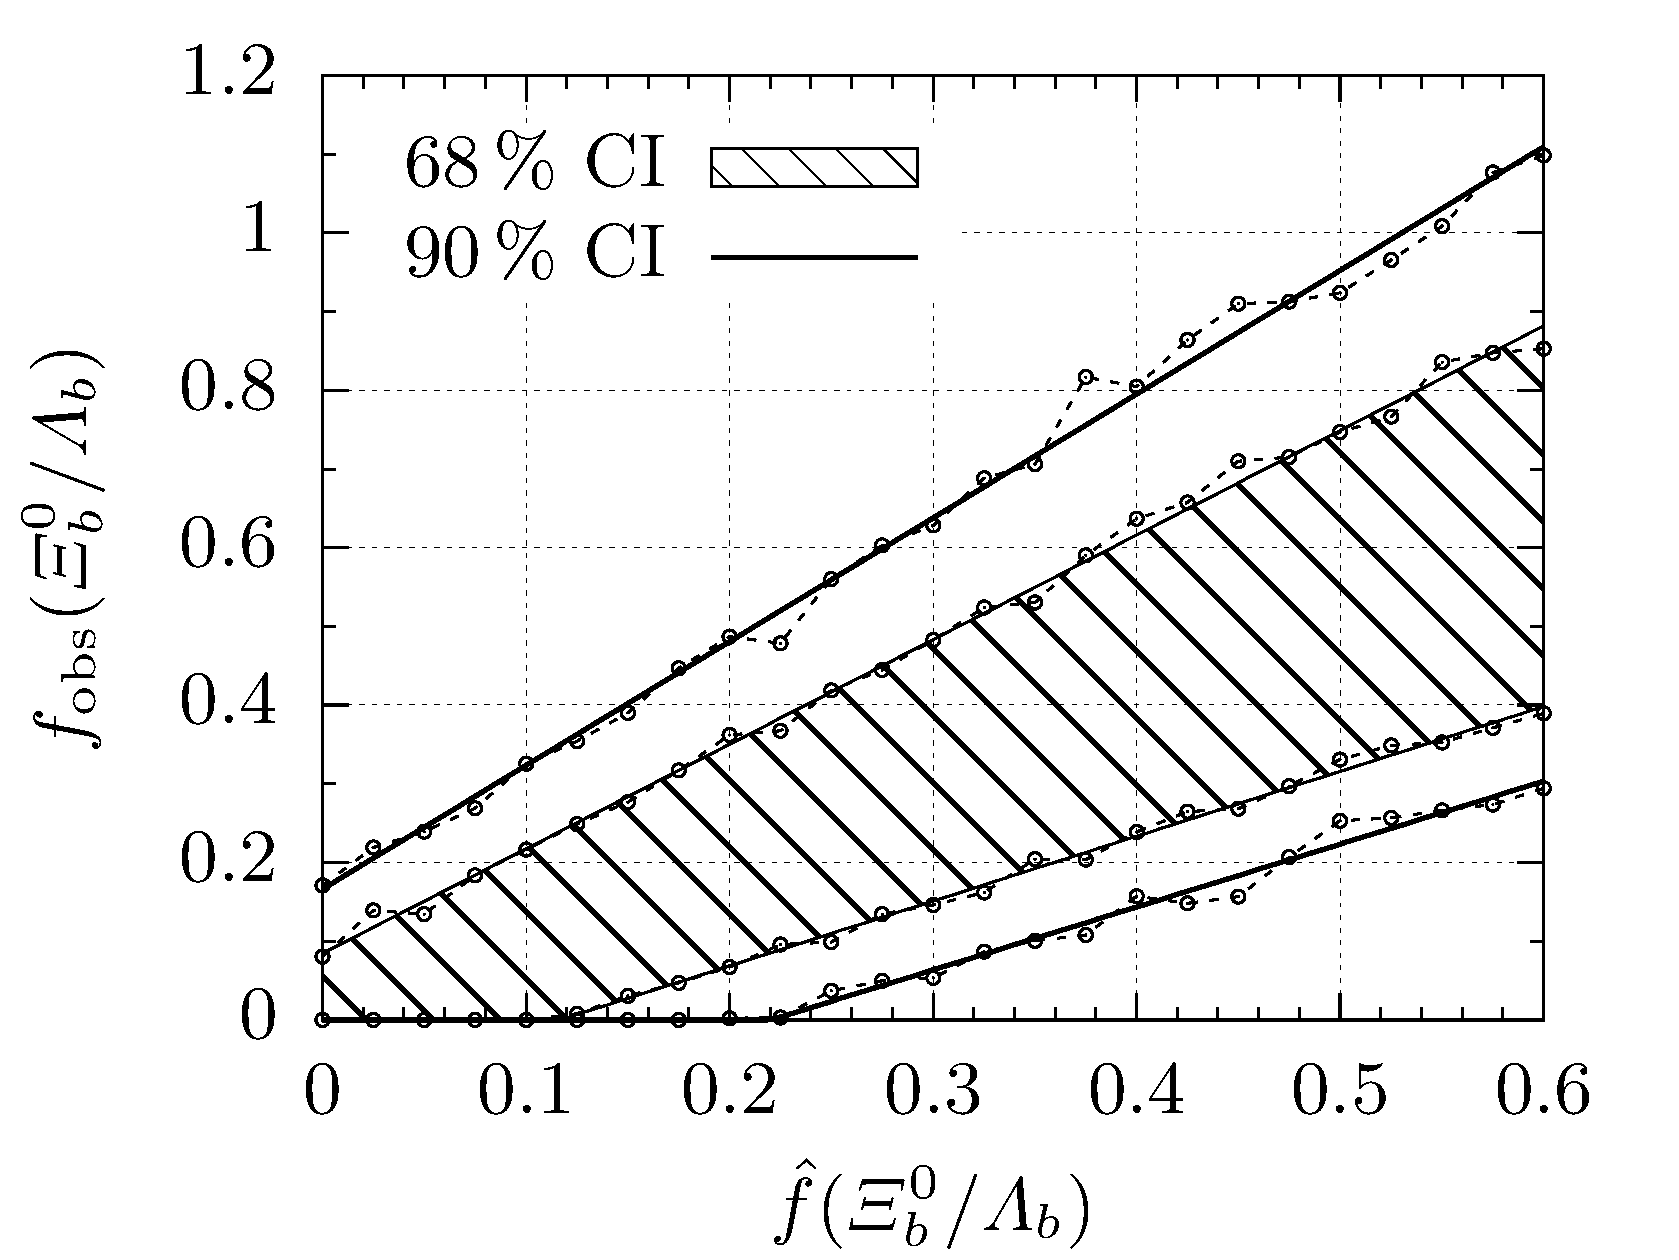
\includegraphics[width=\textwidth]{br/freqci-fit.png}\\
            (central in $f_\text{obs}$)}%
            \only<2>{%
            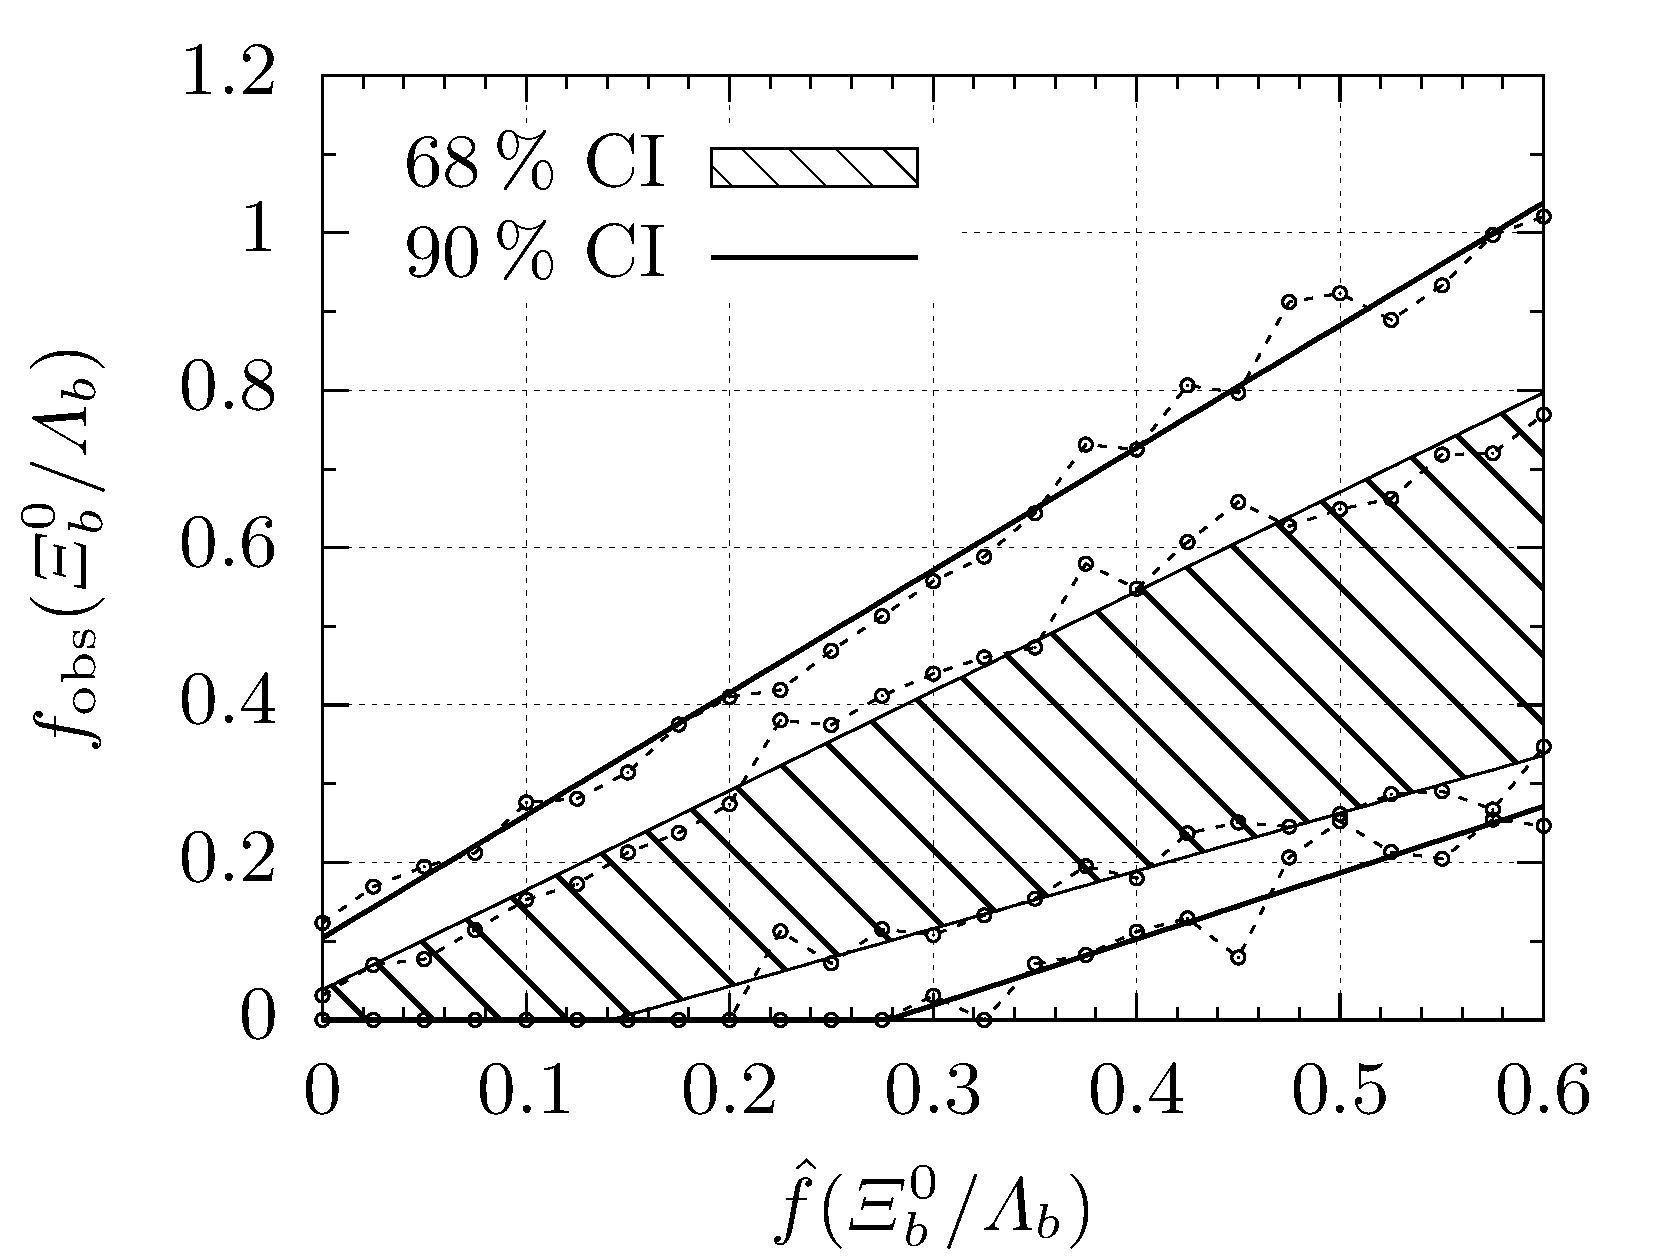
\includegraphics[width=\textwidth]{br/freqci-fit_shortest.png}\\
            (shortest in $f_\text{obs}$)}%
        \end{column}
    \end{columns}
\end{frame}

\begin{frame}{Results / Outlook}
    \begin{columns}
        \begin{column}{.7\textwidth}
            \textbf{Search for new decays}
            \begin{itemize}
                \item \decay{\Lb}{\Dz\Lz} with a stat.\ sign.\ of 5.5$\,\sigma$ (discovery)
                \item \decay{\Xibz}{\Dz\Lz} with a stat.\ sign.\ of 1.8$\,\sigma$
            \end{itemize}

            \textbf{Measurement of branching fractions / ratios}
            \begin{itemize}
                \item $\BR(\decay{\Lb}{\Dz\Lz}) = (9.9 \pm 2.3_\text{stat} \pm 1.6_\text{sys} \pm 1.1_\text{ext}) \times 10^{-6}$
                \item $\frac{f_{\Xibz}}{f_{\Lb}} \times \frac{\BR(\decay{\Xibz}{\Dz\Lz})}{\BR(\decay{\Lb}{\Dz\Lz})} < 0.5 \quad (\text{CL}\,=\,95\,\%)$
            \end{itemize}
            
            \vspace{1mm}

            \textbf{Outlook}
            \begin{itemize}
                \item Collect $\sim$ 20x more data (in reach within next LHC runs)
                \item Benchmark SM by measuring CPV parameter $\gamma$ using suppressed \Dz decays
            \end{itemize}
        \end{column}
        \begin{column}{.3\textwidth}
            \centering
            \only<2>{%
            
\includegraphics[height=1cm]{physik_logo.png}\\
            \vspace{4mm}
            
\includegraphics[height=1cm]{uni_logo.png}\\
            \vspace{4mm}
            
\includegraphics[height=1cm]{lhcb_logo.png}
            \hspace{4mm}
            
\includegraphics[height=1cm]{cern_logo.png}\\
            \vspace{4mm}
            
\includegraphics[height=1cm]{bmbf.png}}
        \end{column}
    \end{columns}

    \vspace{5mm}

    \centering
    \only<1>{\scalebox{1.5}{\vphantom{Thank you for your attention}}}%
    \only<2>{\scalebox{1.5}{Thank you for your attention}}
\end{frame}
